\section{Introduction} \label{sec:introduction}
    \IEEEPARstart{M}{otion} Models parameterise \glss{DVF} in terms of a \gls{SS}. They could be considered as an addition to a standard spatially regularised \gls{MC} technique, as they impose a degree of temporal or gate-wise regularisation. In addition, they also allow obtaining \glss{DVF} for time points/gates, not used to fit the model (as long as a relevant \gls{SS} exists~\cite{McClelland2013}). \glss{MM} have seen attention, particularly in \acrshort{CT}~\cite{Li2007EnhancedModel}, but also \acrshort{MR}~\cite{Manke2002RespiratoryModels, Manber2016JointCorrection.}, however less so in clinical \acrshort{PET}/\acrshort{CT}.
    
    In our previous work~\cite{Whitehead2019ImpactPET, Whitehead2020PET/CTFields, Whitehead2021ComparisonMap}, the possibility of incorporating \glss{MM}, in a \gls{MC} framework, for \gls{NAC} \gls{TOF} \acrshort{PET}, where the reference was set to the position of a breath hold \gls{Mu-Map}, was investigated. %This method could be used to deform both the gates to the reference position as well as the reference position to the gates.
    Our preliminary experiments indicated that the combination of both the \gls{MM} and \gls{TOF}, allowed for an \gls{AC} reconstruction with \gls{MC}, without introducing artefacts, while increasing resolution and quantification accuracy (for simulations with high \gls{TOF} resolution and count levels). This work seeks to extend the method further, using more realistic simulation and count levels, from existing clinical scanners. Firstly, by incorporating \acrshort{MLACF}% as an initialisation technique
    , which provides volumes with greater contrast than \gls{NAC}, without introducing bias due to misalignment with a fixed \gls{Mu-Map}~\cite{Nuyts2012ML-reconstructionFactors}. Secondly, low noise low temporal/gate resolution data is used to fit the \gls{MM}, while high noise high temporal/gate resolution data is used for the output; this potentially allows for reduced misregistration, as well as improving computation time. Thirdly, a diffeomorphic velocity field parameterised registration was used ,which provided \glss{DVF} free from folding.
    
    A method incorporating \glss{MM} for dynamic \acrshort{PET}/\acrshort{CT}, was proposed in~\cite{Chan2018Non-RigidPET}. Additionally, a method incorporating \acrshort{MLACF} for \acrshort{PET}/\acrshort{CT}, was proposed in~\cite{Lu2018RespiratoryData}. The work presented here, differentiates itself, not only by the ways mentioned above, but also by using a \acrshort{2D} \gls{SS} (rather than a \acrshort{1D} \gls{SS}). Thus allowing more general parametrisation of the motion (here in terms of both displacement and velocity). Additionally, the group-wise method, presented here, makes use of an iterative \gls{MC} algorithm, rather than relying only on a pair-wise method.

% \vspace{-0.4cm}

\section{Methods} \label{sec:methods}
    \subsection{\acrshort{XCAT} Volume Generation} \label{sec:xcat_volume_generation}
        \acrshort{XCAT}~\cite{Segars2010} was used to generate $480$ volumes over a \SI{240}{\second} period, using respiratory traces, derived from \acrshort{2D} CINE-\acrshort{MR} patient data. The maximum displacement of \gls{AP} and \gls{SI} motion, was set to \SI{1.2}{\centi\metre} and \SI{2.0}{\centi\metre} respectively. Activity concentrations were derived from a static \acrshort{18F-FDG} patient scan. The \acrlong{FOV} included the base of the lungs, diaphragm, and the top of the liver, with a \SI{20}{\milli\metre} diameter spherical lesion %(smaller than the max displacement due to \gls{RM})
        placed into the base of the right lung (within the maximum displacement due to \acrlong{RM} of the diaphragm).
    
    % \vspace{-0.5cm}
    
    \subsection{\acrshort{PET} Acquisition Simulation} \label{sec:pet_acquisition_simulation}
        \acrshort{PET} acquisitions were simulated (and reconstructed), using \acrshort{STIR}~\cite{Thielemans2012, Nikos2019} through \acrshort{SIRF}~\cite{Ovtchinnikov2017}, to forward project data using the geometry of a \acrshort{GE} Discovery $710$. Attenuation was included using the relevant \glss{Mu-Map} generated by \acrshort{XCAT}. Pseudo-randoms and scatter were added.% Randoms were added by summing a scaled uniform forward projection to the simulation sinogram. Pseudo-scatter was added by summing a scaled and smoothed forward projection of the activity data at each time point to the simulation sinogram. The smoothing parameter was optimised to give scatter with a similar distribution to a GATE gate simulation. A full scatter simulation was not performed due to software limitations.
        
        Noise was simulated, such that data matched an acquisition over \SI{240}{\second}, emulating a standard single bed position acquisition. The count rate was selected to match that of research scans%, i.e. below that of diagnostic clinical scans. This count rate was selected as a 'worst case scenario'
        .
        
        A respiratory \gls{SS} was generated using \gls{PCA}~\cite{Thielemans2011}. The value of this signal, and its gradient, was used for gating. For \gls{MM} estimation, data were initially pseudo-phase gated; the data was displacement and gradient gated into four bins, where each bin was a quadrant centred on the maximum or minimum of the displacement or gradient. %This is useful as it gives a small number of gates while allowing to fit a \acrshort{2D} \gls{MM} (a plane).
        For the purpose of the \gls{MM} fitting, \gls{SS} values were determined for the post-gated data by taking an average of the \gls{SS} values in each bin.
        
    \subsection{\acrshort{MLACF} Image Reconstruction} \label{sec:mlacf_image_reconstruction}
        Data were reconstructed using \acrshort{MLACF}, with seven full iterations and $24$ subsets for the activity update, and $9$ iterations for the attenuation update~\cite{Nuyts2012ML-reconstructionFactors}. \acrshort{MLACF} was initialised using one iteration of \acrshort{MLEM}, where the breath hold \acrshort{CT} was used for \gls{AC}% (the \gls{ACF} were still initialised with all ones), this gave a small improvement to results without introducing bias.
        . Between iterations, the activity volume and \gls{ACF} sinogram were normalised (scaled to the same magnitude as an equivalent volume/sinogram filled with ones), and a small value was added to each voxel%, this was to aid with stabilising the reconstruction
        . A quadratic prior was included in the reconstruction, to promote smoothness of the \gls{ACF} sinogram.
    
    % \vspace{-0.5cm}
    
    \subsection{Registration} \label{sec:registration}
        Before being registered, each volume underwent pre-processing, including; replication of end-slices, smoothing, and standardisation. This pre-processing was only applied to intermediate data, and was not used for the final output of the method.
        
        Group-wise registration was used, where after an initial pair-wise registration step, a new reference volume was resampled. Registration to the new reference volume, followed by another resample, continued for a set number of iterations. NiftyReg~\cite{Modat2010} was used to perform registrations, using a diffeomorphic velocity field B-spline parameterisation. \acrlong{CPG} spacing of the B-spline coefficients, \acrlong{BE} regularisation term weight, and number of iterations were tuned using a grid search.
        
        Between each iteration, the resampled volume was registered to the position of the \gls{Mu-Map}. The \glss{DVF} for both the group-wise registration, and \gls{Mu-Map} registration were composed together to form one final \gls{DVF}.% With the diffeomorphic nature of the registration this would give a \gls{MM} which could generate \glss{DVF} to and from the gates to the \gls{Mu-Map}.
    
    % \vspace{-0.5cm}
    
    \subsection{\acrlong{MM} Estimation} \label{sec:motion_model_estimation}
        \glss{MM} were fit as a direct \acrlong{RCM} on the \glss{CPG}, %from above~\Fref{sec:registration} 
        and the \gls{SS}% from~\Fref{sec:pet_acquisition_simulation}
        . A weighted \acrlong{LR} was used, where the weighting was taken based on the number of counts in each gate. Once a \gls{MM} was fit, new \glss{DVF} were generated for each gate%, using the \gls{SS} values used to fit the \gls{MM}
        . \gls{MM} fitting occurred between iterations%, the \glss{DVF} generated by the \gls{MM} were used to resample the new target volume at each iteration
        .
    
    % \vspace{-0.5cm}
    
    \subsection{\gls{MC} Image Reconstruction with \gls{AC}} \label{sec:mc_image_reconstruction_with_ac}
        Data were re-gated, using the value of \gls{SS}, and its gradient, to gate data into $30$ respiratory bins ($10$ displacement and $3$ gradient bins).
        
        Data were re-reconstructed with \gls{AC}, deforming the \glss{Mu-Map}, using the inverse of the \glss{DVF} determined using the \gls{MM}. %from~\Fref{sec:motion_model_estimation} 
        \acrshort{OSEM} was used, with two full iterations and $24$ subsets (as in clinical practice)~\cite{Hudson1994}. \gls{MC} was then applied, using \glss{DVF} determined using the \gls{MM}%from~\Fref{sec:motion_model_estimation}
        . Volumes were post-filtered using a Gaussian smoothing, with a \acrshort{FWHM} of \SI{6.4}{\milli\metre} in the transverse plane, and a normal Z-filter (as in clinical practice).
    
    % \vspace{-0.5cm}
    
    \subsection{Evaluation} \label{sec:evaluation}
        In addition to the reconstructions performed %in~\Fref{sec:motion_corrected_image_reconstruction_with_ac}, 
        above, data were also \gls{MC} in the same way, %as in~\Fref{sec:registration} and~\Fref{sec:motion_model_estimation} 
        but using high noise high temporal/gate resolution, or noiseless data, for the \gls{MM} fitting. Furthermore, data were also reconstructed without \gls{MC}, using either the end inhalation \gls{Mu-Map}, or a sum of all \glss{Mu-Map} (to emulate an \gls{AV-CCT}). For the present evaluation, the volumes without \gls{MC} were registered to the position of the end inhalation \gls{Mu-Map}. Additionally, \glss{DVF} generated by each method were also applied to the original \acrshort{XCAT} volumes, for visual analysis.
        
        Comparisons used included: A visual analysis, \acrshort{SSIM} to the ground truth~\cite{Wang2009MeanMeasures}, a profile over the lesion, and \acrshort{SUV}\textsubscript{max} and \acrshort{SUV}\textsubscript{peak} (defined following \acrshort{EANM} guidelines~\cite{Boellaard2015FDG2.0}).

% \vspace{-0.5cm}

\section{Results} \label{sec:results}
    \begin{figure*}
        % \vspace{-0.5cm}
        
        \centering
        
        % 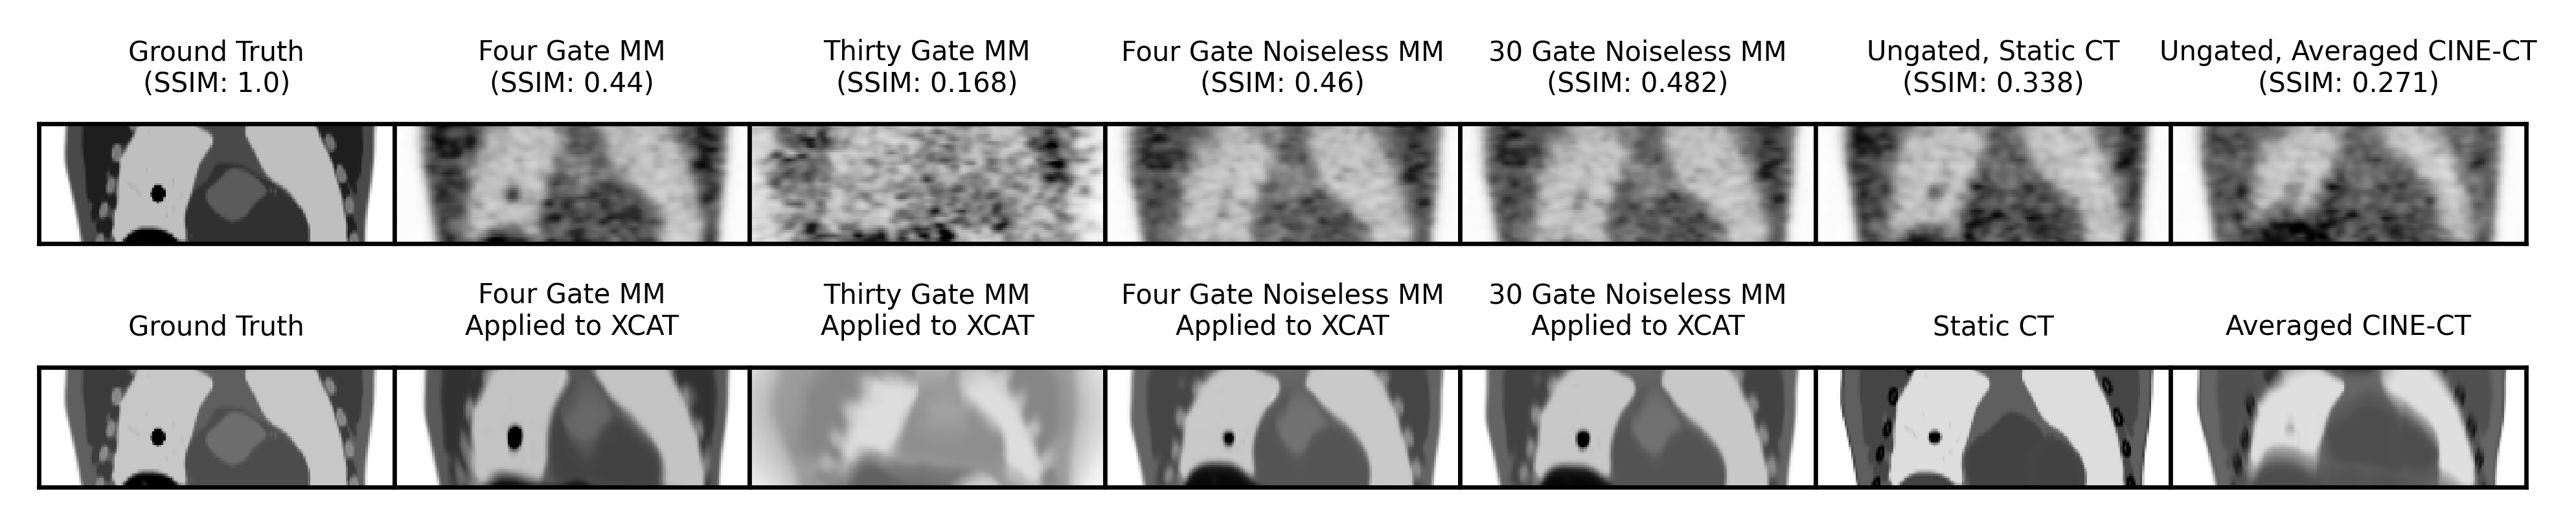
\includegraphics[width=0.93\linewidth]{figures/visual_analysis.png}
        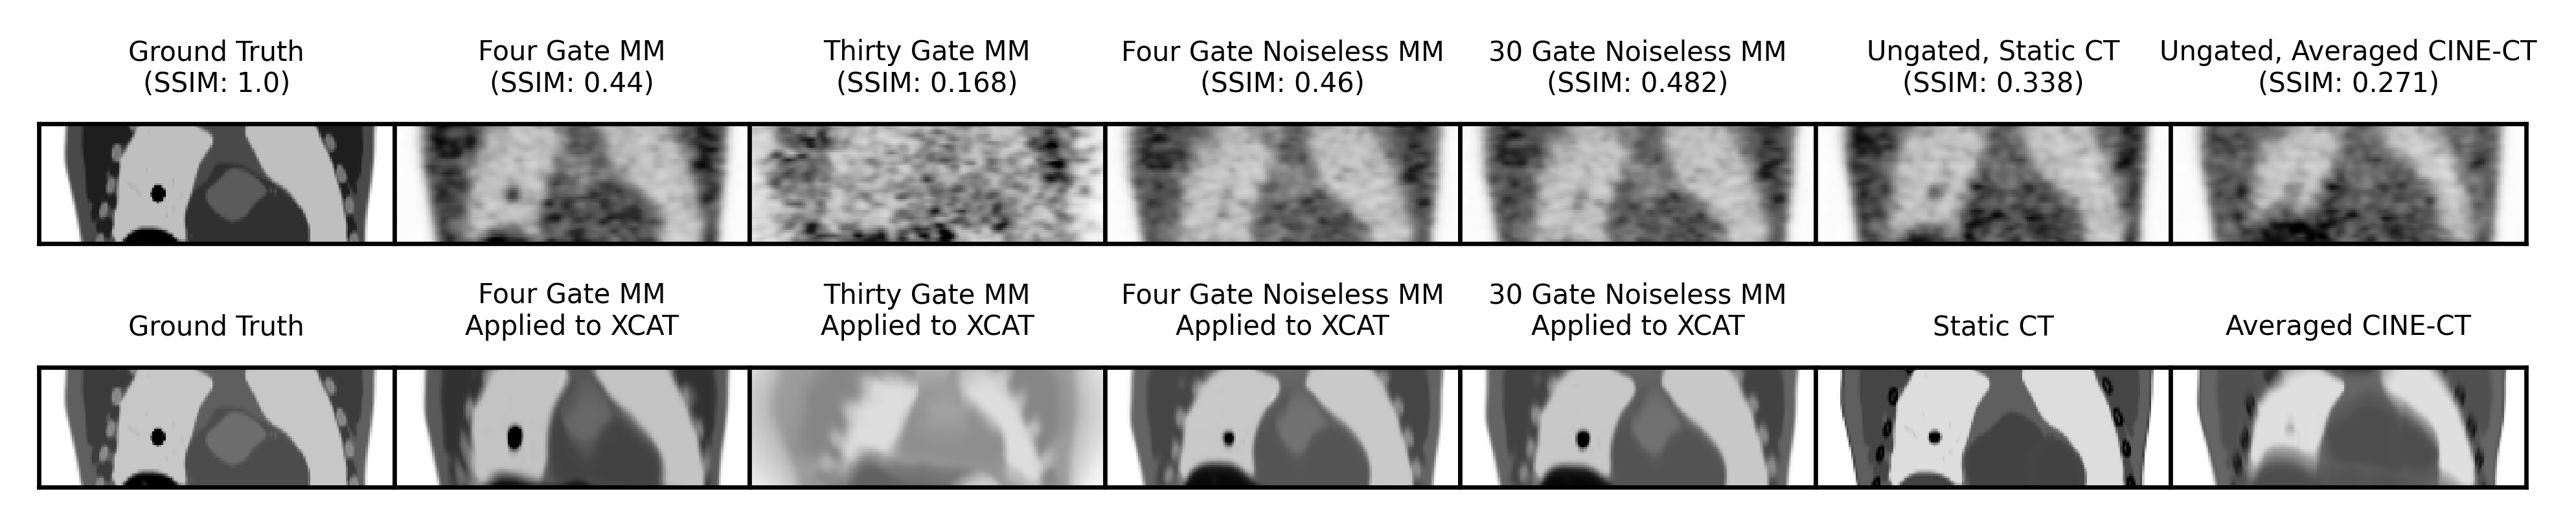
\includegraphics[width=1.0\linewidth]{figures/visual_analysis.png}
        
        % \vspace{-0.5cm}
        
        \captionsetup{singlelinecheck=false, justification=centering}
        \caption{
        % \scriptsize
        First row contains, \gls{AC} \gls{MC} reconstructions (plus \acrshort{SSIM} to the ground truth), and the second row contains, the results of applying the final \gls{MM} on the original \acrshort{XCAT} volumes, with the ground truth \acrshort{XCAT} data (for both activity and attenuation), for; a \gls{MM} fit on four and $30$ gate binned data applied to $30$ gate binned data, a \gls{MM} fit on noiseless four and $30$ gate binned data applied to $30$ gate binned data, and ungated data \gls{AC} with a static \gls{Mu-Map} at end inhalation and all \glss{Mu-Map} summed. Colour map ranges are consistent for all images in each row.}
        
        \label{fig:visual_analysis}
        
        % \vspace{-0.5cm}
    \end{figure*}
    
    \begin{figure}
        % \vspace{-0.5cm}
        
        \centering
        
        % 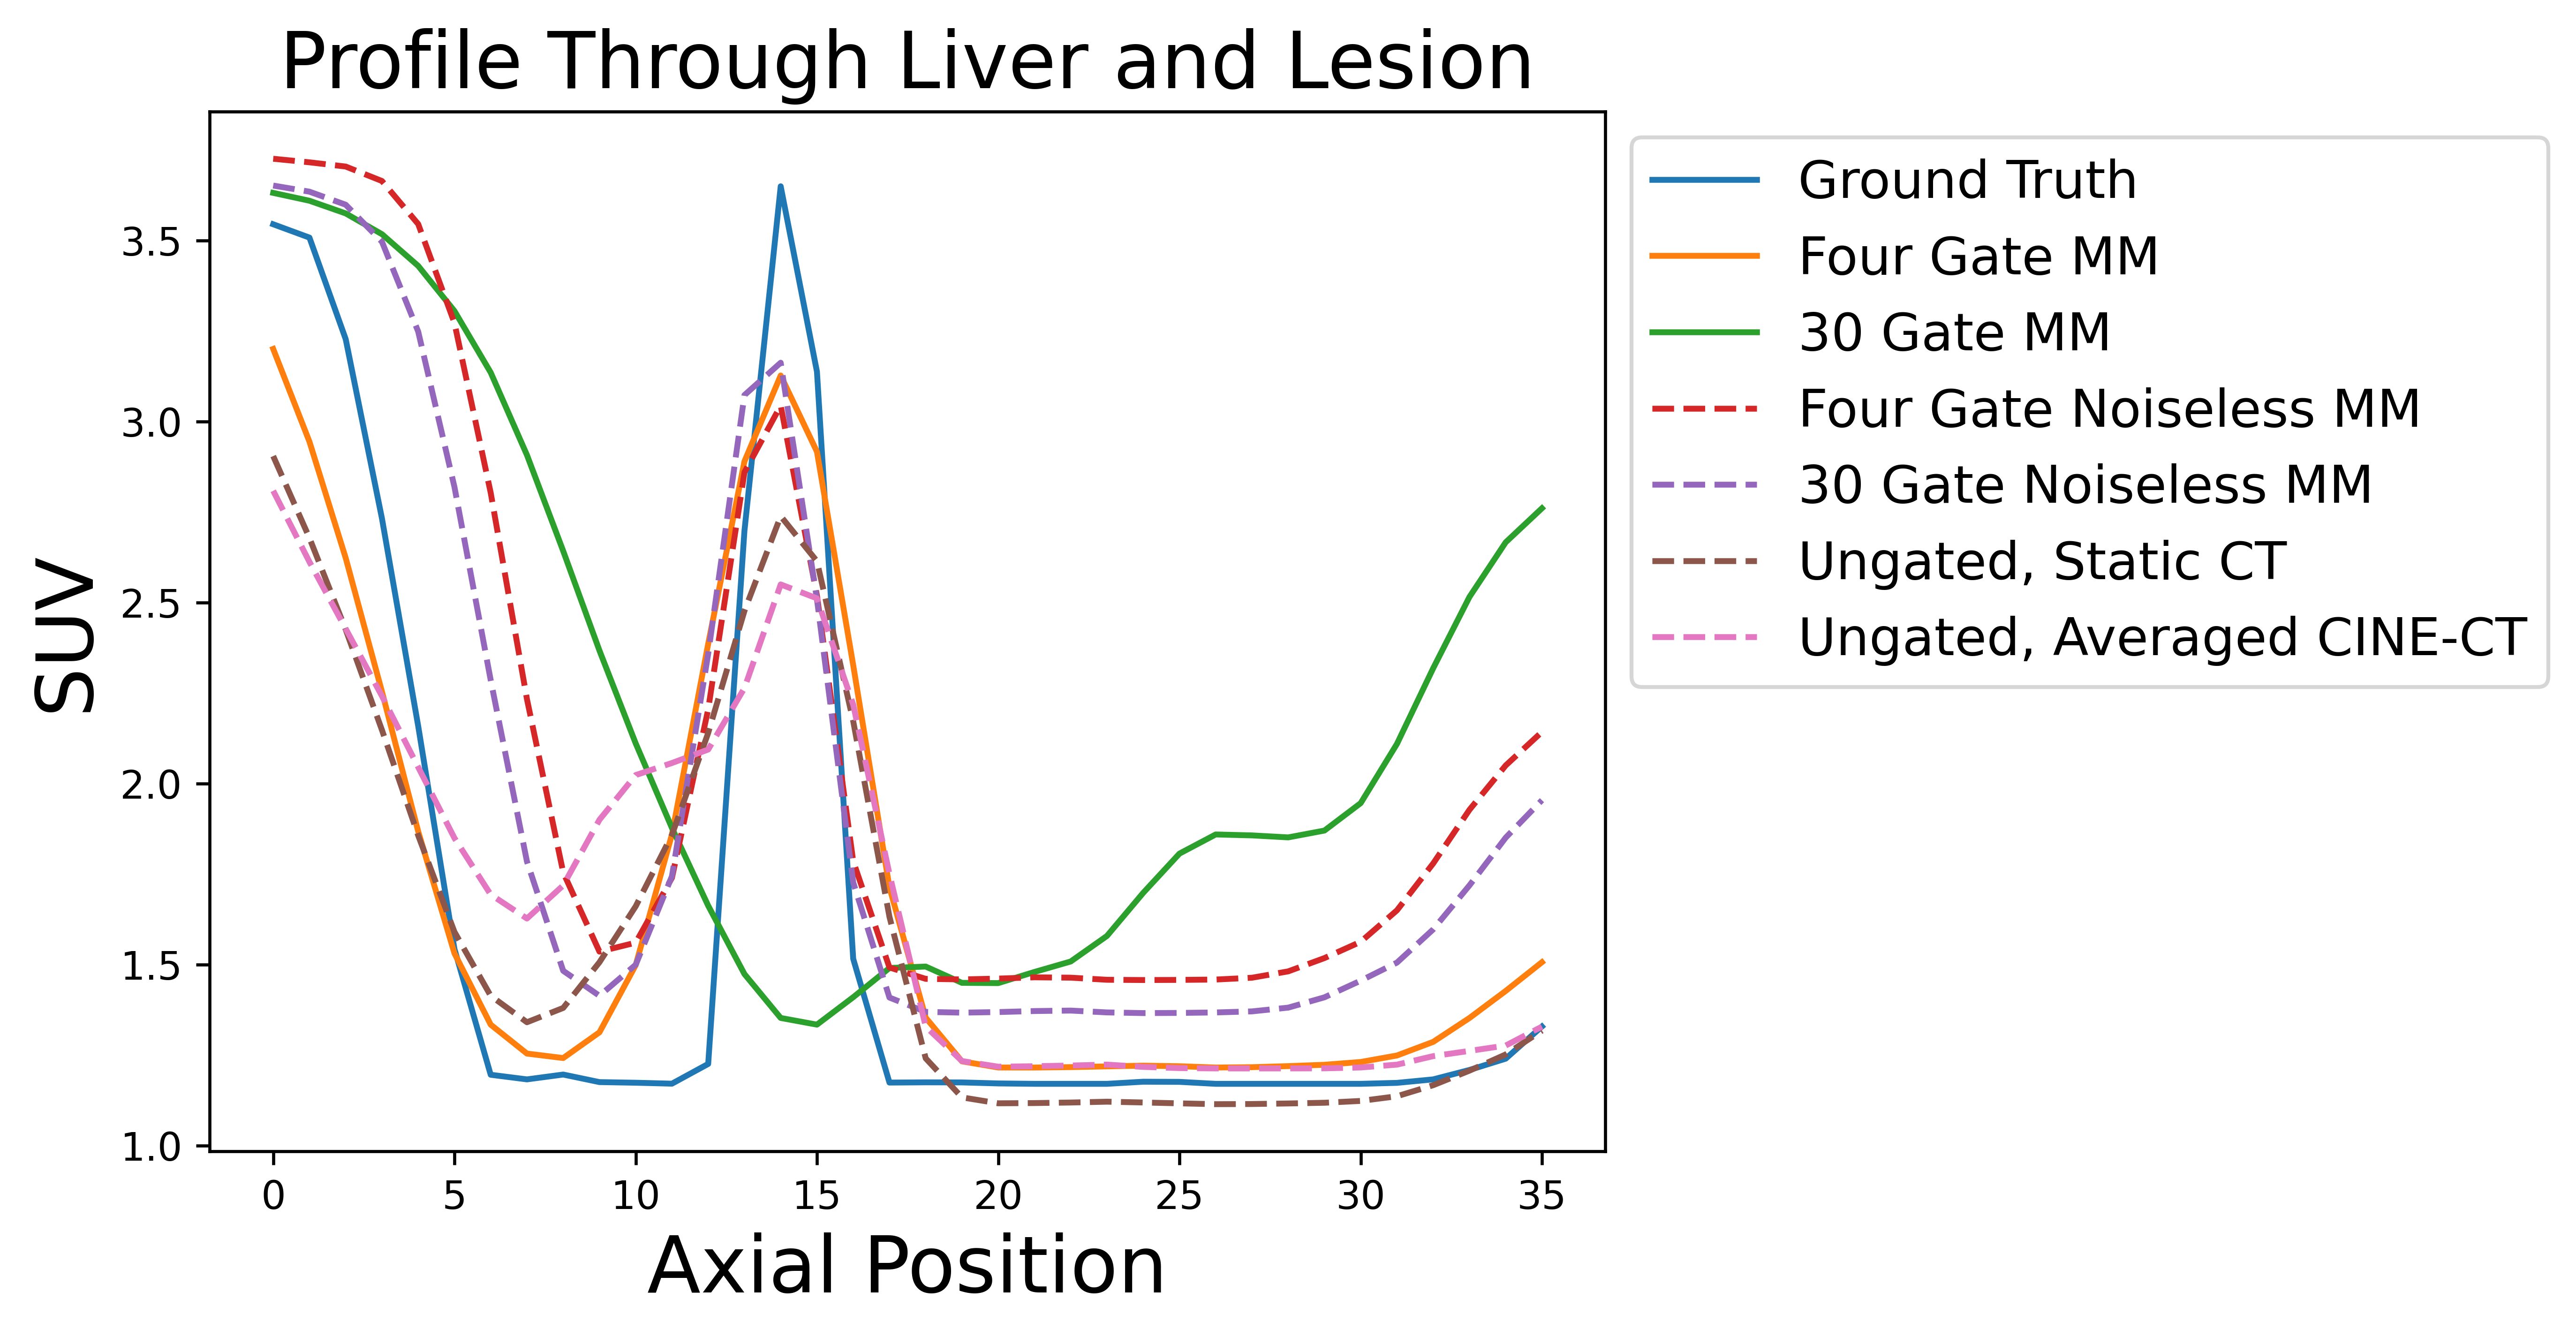
\includegraphics[width=0.93\linewidth]{figures/profile.png}
        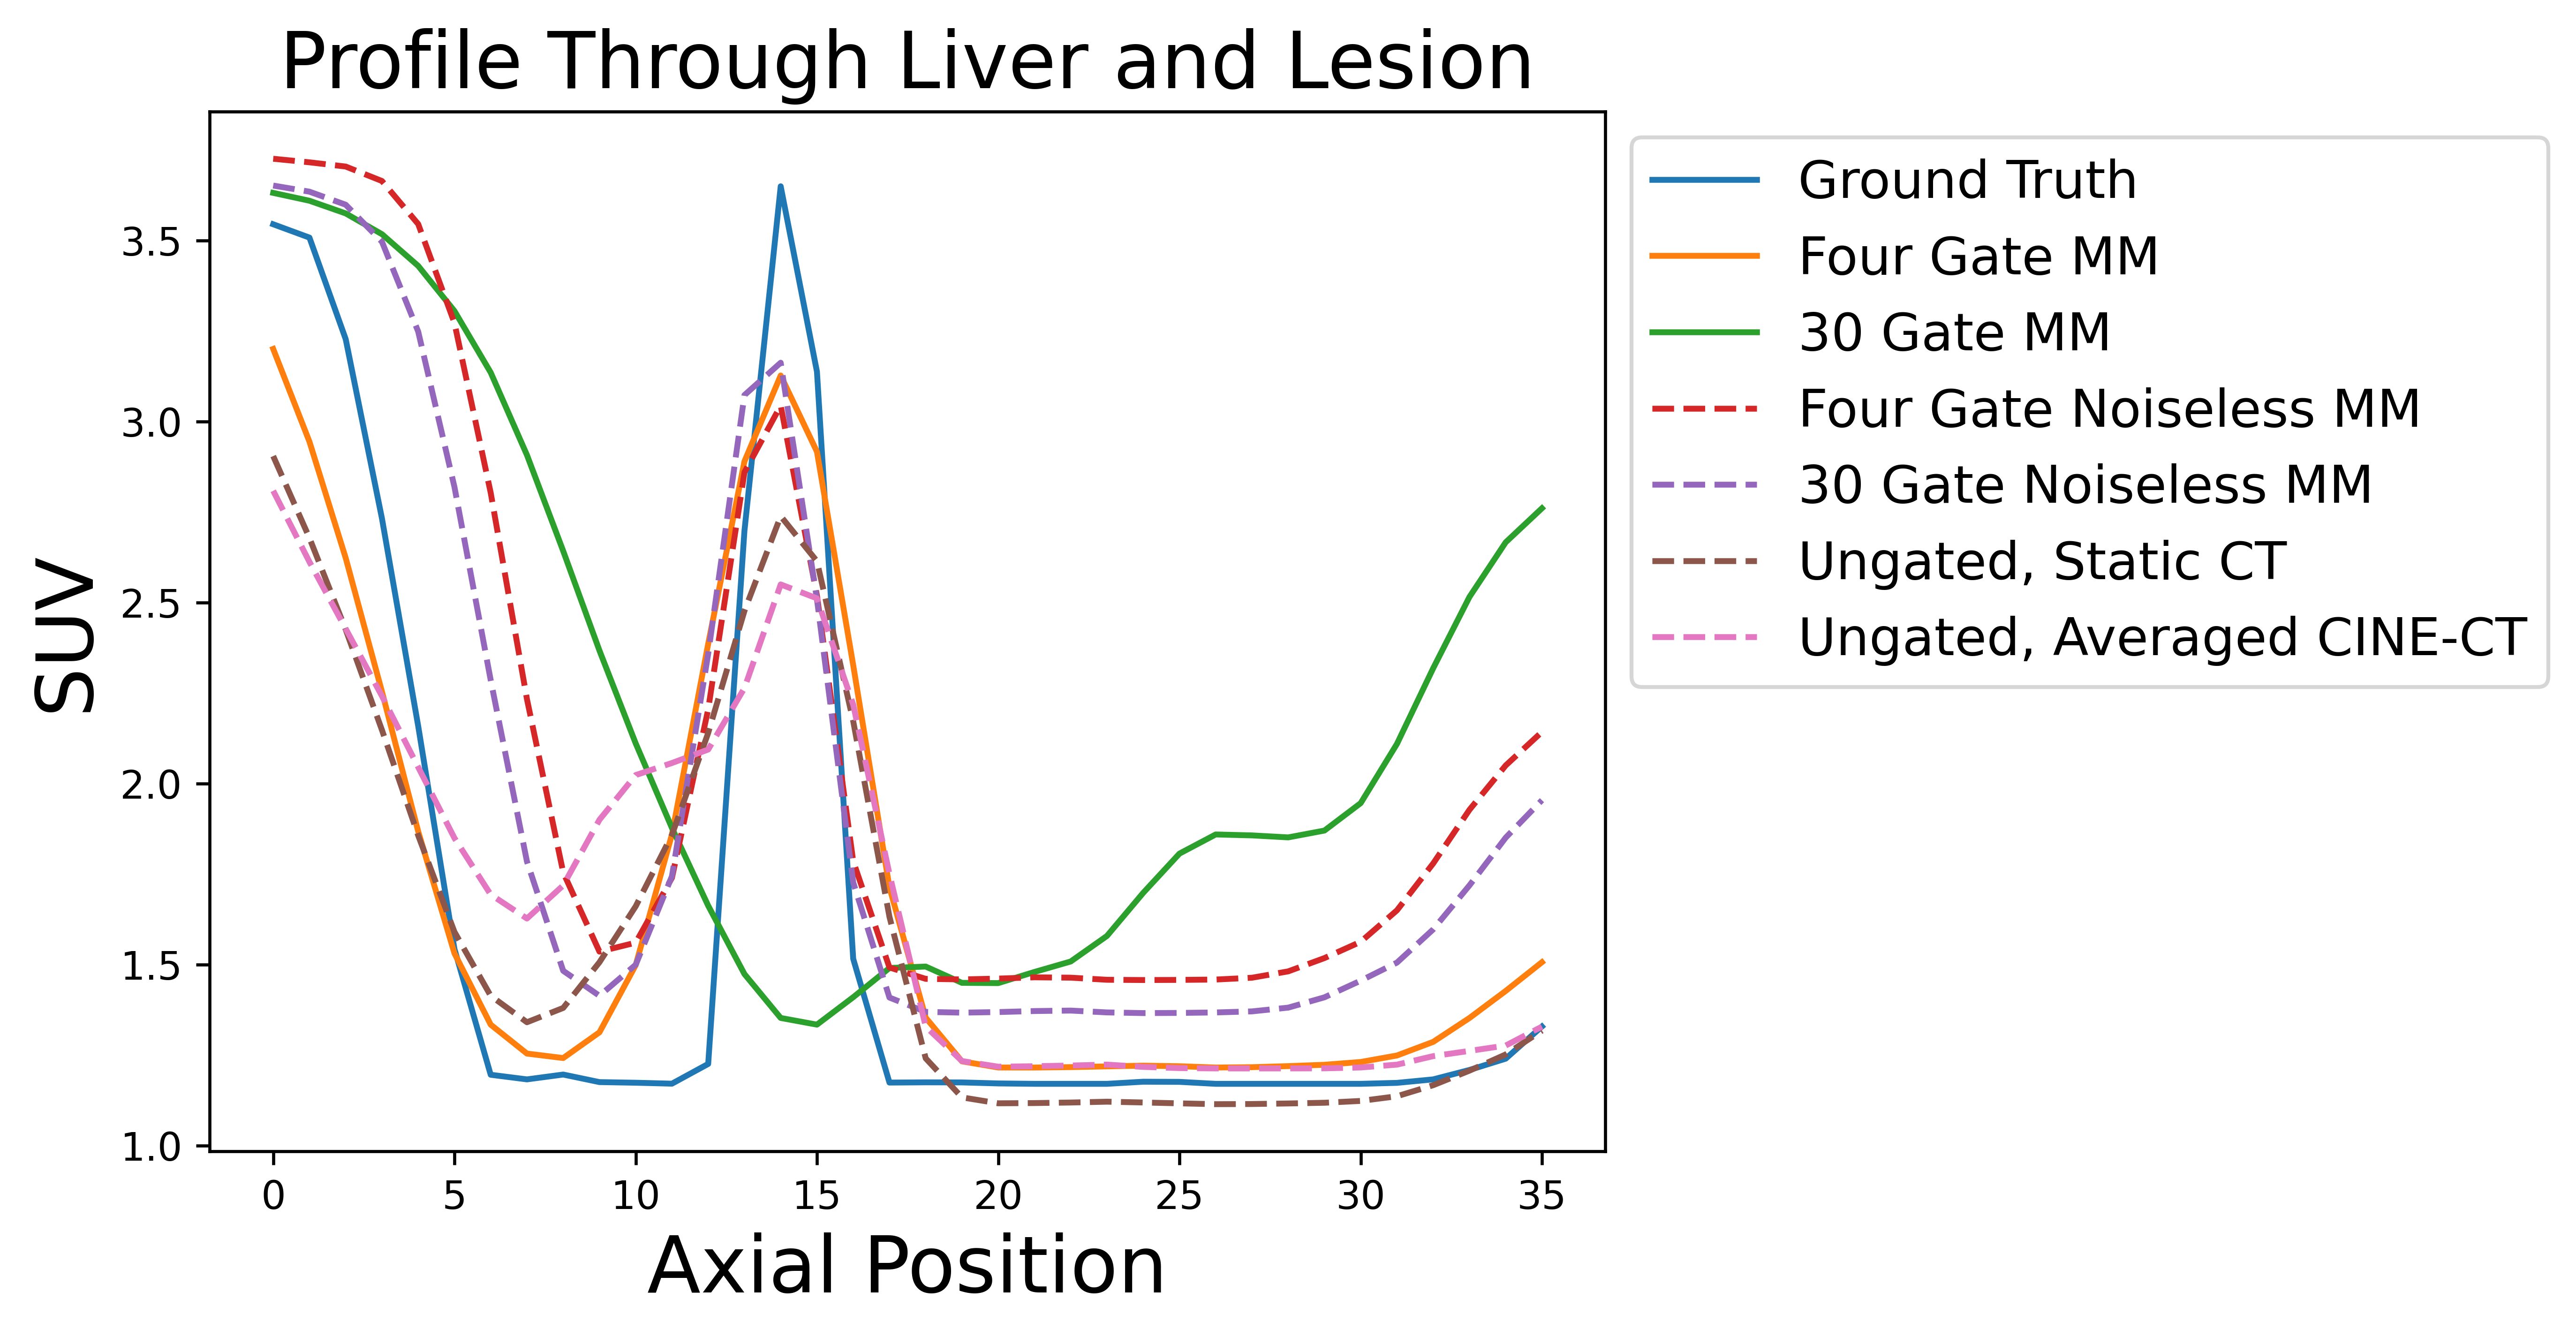
\includegraphics[width=1.0\linewidth]{figures/profile.png}
        
        % \vspace{-0.5cm}
        
        \captionsetup{singlelinecheck=false, justification=centering}
        \caption{
        % \scriptsize
        A profile through the lesion, in the \gls{SI} direction, summed over a window in the \gls{AP} and \acrlong{LM} directions, with median smoothing, for; the ground truth \acrshort{XCAT} data, a \gls{MM} fit on four and $30$ gate binned data applied to $30$ gate binned data, a \gls{MM} fit on noiseless four and $30$ gate binned data applied to $30$ gate binned data, and ungated data \gls{AC} with a static \gls{Mu-Map} at end inhalation and all \glss{Mu-Map} summed.}
        
        \label{fig:profile}
        
        % \vspace{-0.5cm}
    \end{figure}
    
    \begin{table}
        % \vspace{-0.5cm}
        
        \centering
        
        \captionsetup{singlelinecheck=false, justification=centering}
        \caption{
        % \tiny
        Comparison of \acrshort{SUV}\textsubscript{max} and \acrshort{SUV}\textsubscript{peak}, for; the ground truth \acrshort{XCAT} data, a \gls{MM} fit on four and $30$ gate binned data applied to $30$ gate binned data, a \gls{MM} fit on noiseless four and $30$ gate binned data applied to $30$ gate binned data, and ungated data \gls{AC} with a static \gls{Mu-Map} at end inhalation and all \glss{Mu-Map} summed.}
        
        % \vspace{-0.5cm}
        
        % \resizebox*{0.6\linewidth}{!}
        \resizebox*{1.0\linewidth}{!}
        {
            \begin{tabular}{||c|cc||}
                \hline
                \textbf{\acrshort{SUV}}                 & \textbf{Max}  & \textbf{Peak} \\
                \hline
                \textbf{Ground Truth}                   & $8.76$        & $7.96$ \\
                \hline
                \textbf{Four Gate \gls{MM}}             & $8.04$        & $6.18$ \\
                \textbf{30 Gate \gls{MM}}               & $1.77$        & $1.32$ \\
                \hline
                \textbf{Four Gate Noiseless \gls{MM}}   & $8.05$        & $6.24$ \\
                \textbf{30 Gate Noiseless \gls{MM}}     & $7.96$        & $5.99$ \\
                \hline
                \textbf{Ungated, Static \acrshort{CT}}  & $6.61$        & $5.08$ \\
                \textbf{Ungated, \gls{AV-CCT}}          & $5.65$        & $4.44$ \\
                \hline
            \end{tabular}
        }
        \label{tab:suv}
        
        % \vspace{-0.5cm}
    \end{table}
    
    A visual comparison of the reconstructed images (see~\Fref{fig:visual_analysis}), shows that the high noise high temporal/gate resolution method performs quite poorly, most probably due to the high level of noise apparent in the volumes. Conversely, the low noise low temporal/gate resolution data method appears to be able to \gls{MC} the data without being too adversely affected by the noise level.
     
    The peak of the profile (see~\Fref{fig:profile}) for the four gate \gls{MM} results is comparable to the noiseless results. In contrast, the $30$ gate \gls{MM} method fails on the noisy data. For all other \gls{MC} methods, the peak is greater than without \gls{MC}.
     
    \acrshort{SUV} (and \acrshort{SSIM}) results confirm the above (see~\Fref{tab:suv}).

% \vspace{-0.4cm}

\section{Discussion and Conclusions} \label{sec:discussion_and_conclusions}
    Results show that using a low number of gates for \gls{MM} fitting, has minimal impact at low noise, while improving \gls{MC} when there is a high level of noise in the gates. In addition, the execution time using a reduced number of gates is lower.
    
    In the future, work will focus on evaluating the method on patient data.
    